\documentclass[twoside, a4paper]{article}
\usepackage{graphicx}
\usepackage[spanish]{babel}
\begin{document}
1)Planificaci\'on FCFS:\\
\begin{figure*}[!htb]
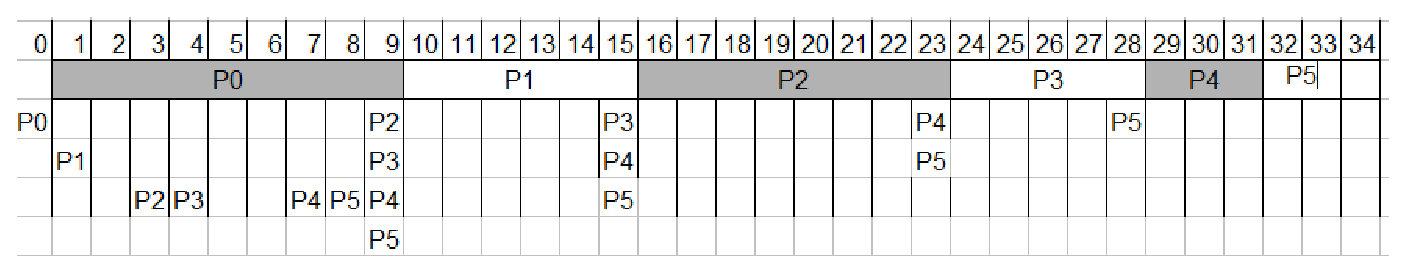
\includegraphics[scale=0.60]{FCFS.eps}
\end{figure*}
\begin{tabular}{l l}
Tiempos de retorno & Tiempo de espera\\
$P_0 =-(0 - 9)= 9$ & $P_0 = 0$ \\
$P_1 =-(1 - 15)= 14$ & $P_1 =10-1=9$ \\
$P_2 =-(3 - 23)= 20$ & $P_2 =16-3=13$\\
$P_3 =-(4 - 28)= 24$ & $P_3 =24-4=20$\\
$P_4 =-(7 - 31)= 24$ & $P_4 =29-7=22$\\
$P_5 =-(8 - 33)= 25$ & $P_5 =32-8=24$\\
Tiempo promedio = 19,33 & 14,66
\end{tabular}
\newline
Prioridad No Apropiativo:\\
\begin{figure*}[!htb]
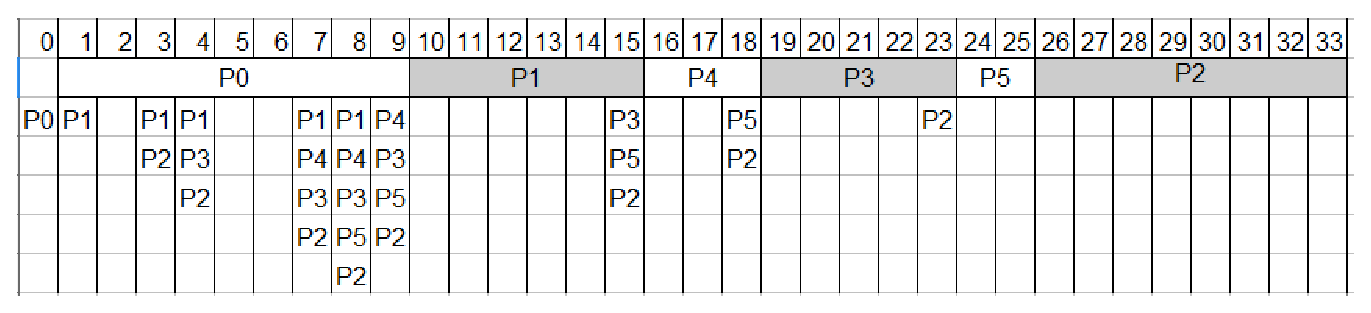
\includegraphics[scale=0.60]{Prioridad-noApropiativo.eps}
\end{figure*}
\begin{tabular}{l l}
Tiempos de retorno & Tiempo de espera\\
$P_0 =-(0 - 9)= 9$   & $P_0 = 0$ \\
$P_1 =-(1 - 15)= 14$ & $P_1 = 10-1= 9$ \\
$P_2 =-(3 - 33)= 30$ & $P_2 = 26-3= 23$\\
$P_3 =-(4 - 23)= 19$ & $P_3 = 19-4= 15$\\
$P_4 =-(7 - 18)= 11$ & $P_4 = 16-7= 9$\\
$P_5 =-(8 - 25)= 17$ & $P_5 = 24-8= 16$\\
Tiempo promedio = 16,66 & 12
\end{tabular}
\newline
SJF No Apropiativo:\\
\begin{figure*}[!htb]
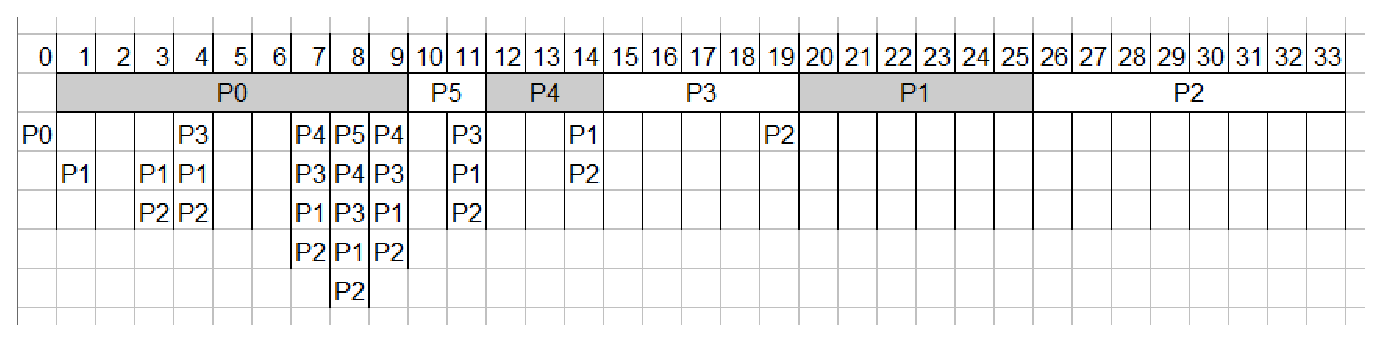
\includegraphics[scale=0.60]{SJF-noApropiativo.eps}
\end{figure*}
\begin{tabular}{l l}
Tiempos de retorno & Tiempo de espera\\
$P_0 =-(0 - 9)= 9$   & $P_0 = 0$ \\
$P_1 =-(1 - 25)= 24$ & $P_1 = 20-1= 19$ \\
$P_2 =-(3 - 33)= 30$ & $P_2 = 26-3= 23$\\
$P_3 =-(4 - 19)= 15$ & $P_3 = 15-4= 11$\\
$P_4 =-(7 - 14)= 7$ & $P_4 = 12-7= 5$\\
$P_5 =-(8 - 11)= 3$ & $P_5 = 10-8= 2$\\
Tiempo promedio = 14,66 & 10
\end{tabular}


Prioridad Apropiativo:\\
\begin{figure*}[!htb]
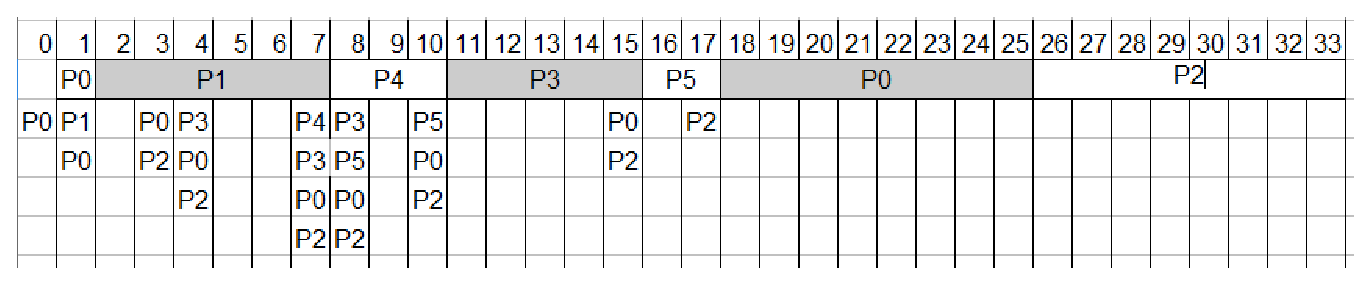
\includegraphics[scale=0.60]{Prioridad-Apropiativo.eps}
\end{figure*}
\begin{tabular}{l l}
Tiempos de espera 		 & Tiempo de retorno\\
$P_0 = 6+(18 - 2)= 16$   & $P_0 = 25-0 = 0$ \\
$P_1 = 1 - 1= 0$ 		 & $P_1 = 7-1= 6$ \\
$P_2 =-(3 - 26)= 23$ 	 & $P_2 = 33-3= 30$\\
$P_3 =-(4 - 11)= 9$ 	 & $P_3 = 15-4= 11$\\
$P_4 = 0$ 				 & $P_4 = 10-7= 3$\\
$P_5 =-(8 - 16)= 8$ 	 & $P_5 = 17-8= 9$\\
Tiempo promedio = 9,33 	 & 14
\end{tabular}
\newline
SJF Apropiativo:\\
\begin{figure*}[!htb]
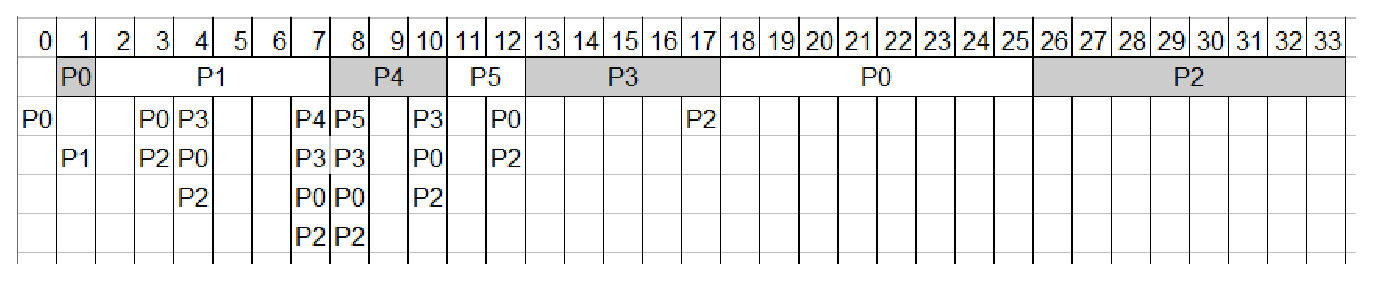
\includegraphics[scale=0.60]{SJF-Apropiativo.eps}
\end{figure*}
\begin{tabular}{l l}
Tiempos de retorno 		& Tiempo de espera\\
$P_0 =-(0 - 25)= 25$   	& $P_0 = 18-1= 17$ \\
$P_1 =-(1 - 7)= 6$ 		& $P_1 = 0$ \\
$P_2 =-(3 - 33)= 30$ 	& $P_2 = 26-3= 23$\\
$P_3 =-(4 - 17)= 13$ 	& $P_3 = 13-4= 9$\\
$P_4 =-(7 - 10)= 3$ 	& $P_4 = 7-7= 0$\\
$P_5 =-(8 - 12)= 4$ 	& $P_5 = 11-8= 3$\\
Tiempo promedio = 13,5 	& 8,66
\end{tabular}
\newline
\newline
Round Robin:\\
\begin{figure*}[!htb]
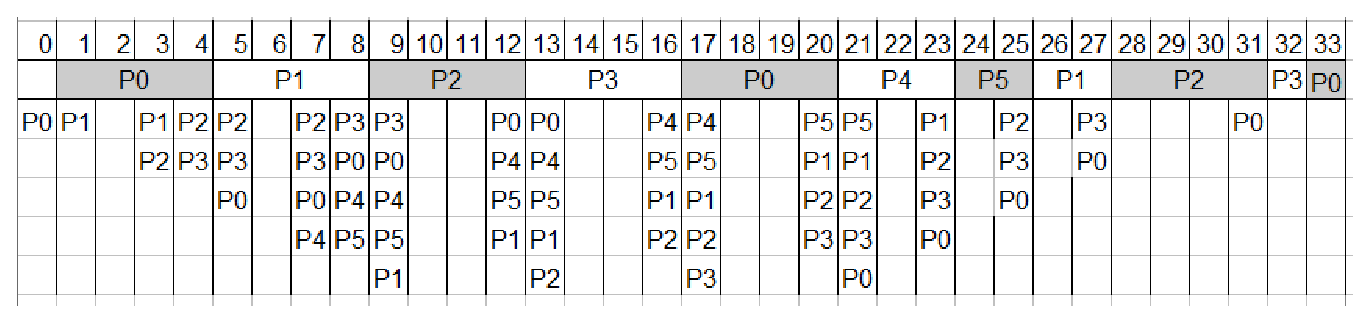
\includegraphics[scale=0.60]{Round-Robin.eps}
\end{figure*}
\begin{tabular}{l l}
Tiempos de retorno 		& Tiempo de espera\\
$P_0 = 33$   		 	& $P_0 = 0$ \\
$P_1 =-(1 - 27)= 26$ 	& $P_1 = 20-1= 19$ \\
$P_2 =-(3 - 31)= 28$ 	& $P_2 = 26-3= 23$\\
$P_3 =-(4 - 32)= 28$ 	& $P_3 = 15-4= 11$\\
$P_4 =-(7 - 23)= 16$ 	& $P_4 = 12-7= 5$\\
$P_5 =-(8 - 25)= 17$ 	& $P_5 = 10-8= 2$\\
Tiempo promedio = 14,66 & 10
\end{tabular}
\end{document}
